%-------------------------------------------------------------------------------
% cookbook_presets
%-------------------------------------------------------------------------------
%
% \file        cookbook_presets.tex
% \library     Documents
% \author      Chris Ahlstrom
% \date        2016-03-09
% \update      2016-03-10
% \version     $Revision$
% \license     $XPC_GPL_LICENSE$
%
%     Provides a tutorial on presets.
%
%-------------------------------------------------------------------------------

\section{Fun With Presets}
\label{sec:presets}

   This section expands on its counterpart in the  \textsl{Yoshimi User Manual},
   showing how presets can be employed to re-use blocks of settings.
   In this short tutorial, we will grab and save a number of presets,
   and then use them to partly reconstitute the sound.

\subsection{Presets / Paths}
\label{subsec:presets_paths}

   First, one needs to make sure to have one's
   \texttt{\textasciitilde/.config/yoshimi/presets} directory
   in the set of preset directories.
   Navigate to the \textbf{Main window / Paths / Preset Dirs...} menu entry
   and see if it is there.
   Add it if necessary.

   Second, make sure that there are some root directories available.
   Navigate to the \textbf{Main window / Paths / Bank Root Dirs...} menu entry
   and make sure at least the first of these directories are present:

   \begin{verbatim}
      /usr/share/yoshimi/banks (or in /usr/local if built from source)
      /usr/share/zynaddsubfx/banks
   \end{verbatim}

\subsection{Presets / Pick a Patch}
\label{subsec:presets_pick_a_patch}

   Now navigate to
   \textbf{Main window / Patch Sets / Show Patch Banks...}.
   Pick item \textbf{60. Pads}.
   In the Pads bank window that opens, pick \textbf{8. Resonance Pad1}.
   The following figure shows the set of windows that are now open:

\begin{figure}[H]
   \centering 
   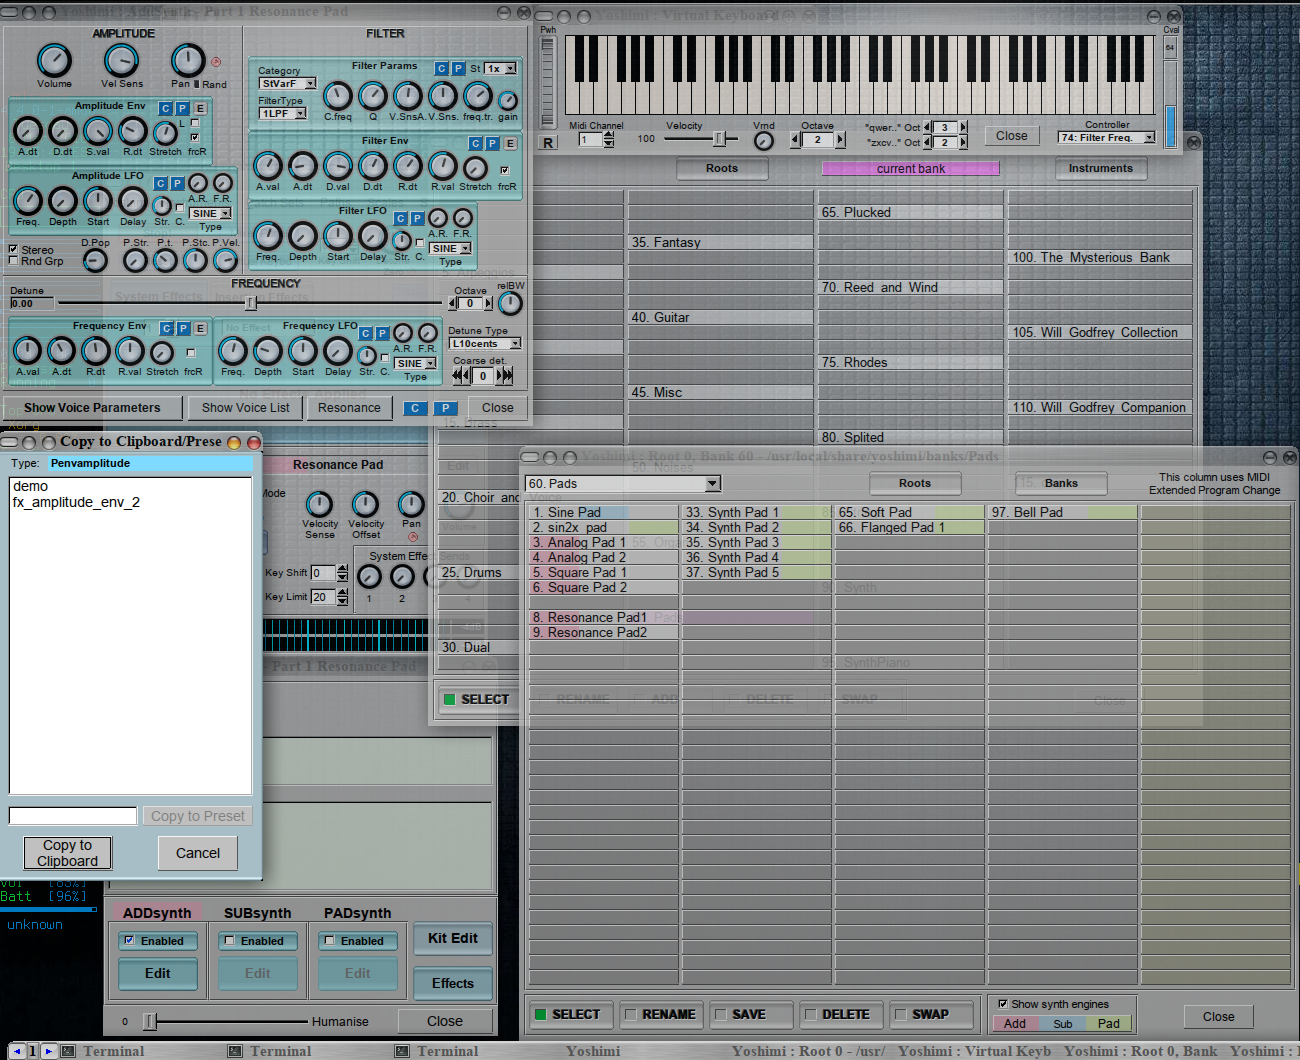
\includegraphics[scale=0.5]{navigating-to-a-preset.png}
   \caption{Navigating to a Preset}
   \label{fig:presets_navigating_to_a_preset}
\end{figure}

   Take a moment to note each of the windows that are open now.
   Play the virtual keyboard for awhile, until the sound of this
   patch/instrument is memorized (we want to reconstruct this sound later).

   Now let's save some of the instrument's presets.
   Click the \textsl{Yoshimi} main window's \textbf{Edit} button.
   Oddly, this PAD instrument uses only the ADDsynth engine.
   Press the ADDsynth item's \textbf{Edit} button.
   Up comes the complex, multi-panelled window for the ADDsynth setup.
   Note the blue \textbf{C} and \textbf{P} buttons in each of the following
   sub-panels:

   \begin{itemize}
      \item \textbf{Amplitude Env}
      \item \textbf{Amplitude LFO}
      \item \textbf{Filter Params}
      \item \textbf{Filter Env}
      \item \textbf{Filter LFO}
      \item \textbf{Frequency Env}
      \item \textbf{Frequency LFO}
      \item The whole \textbf{ADDsynth Window}
   \end{itemize}

   Let's save them all!  Click on each \textbf{C} button,
   then fill in the \textbf{Copy to Preset} text field with
   the name \textsl{"demo"}, and then press the \textbf{Copy to Preset}
   button.  All of the file-names that result will start with
   \texttt{demo}.

   Then click on the \textbf{Show Voice Parameters} button,
   then click on the \textbf{C} button to save the one enabled sub-panel
   for that instrument's voice, \textbf{Frequency LFO}.
   Note that the \textsl{demo} is already saved in this preset of
   type \textsl{Plfofrequency}.  So, if we want to save this, we'd use a
   name other than \textsl{demo}.  Click \textbf{Cancel}.

   Now click on the \textbf{C} button
   for the whole ADDsynth voice window.  Go ahead and do
   \textbf{Copy to Preset} named "demo".

   Now look in \texttt{\textasciitilde/.config/yoshimi/presets}",
   and see all the saved files:

\begin{verbatim}
	$ ls ~/.config/yoshimi/presets
	demo.ADnoteParametersn.xpz (whole ADDsynth preset?)
	demo.ADnoteParameters.xpz (whole ADDsynth Voice preset?)
	demo.Penvamplitude.xpz
	demo.Penvfilter.xpz
	demo.Penvfrequency.xpz
	demo.Pfilter.xpz
	demo.Plfoamplitude.xpz
	demo.Plfofilter.xpz
	demo.Plfofrequency.xpz
\end{verbatim}

	Two of them are confounded with the same type, but slightly
   different file-names.  How?

   Now all of these presets are available for loading.
   Let's use them to take a basic sine wave, and build up its settings until
   we have something approximating the \textbf{8. Resonance Pad1} sound.
   Let's try to reconstruct the sound.
   
   Load the \textsl{Yoshimi} \textbf{Simple Sound}. 
   This sound currently cannot be obtained via \textbf{Instruments / Clear}!
   (Bug?)
   Therefore just move to the next part number in the main window.
   Or restart \textsl{Yoshimi}.
   Listen to \textbf{Simple Sound} via the virtual keyboard, and note
   how pure and tone-like it is.
   Then click the main window \textbf{Edit} button, then the
   ADDsynth \textbf{Edit} button.
   Now load all of the presets above by clicking on each \textbf{P}
   button and then selecting the \texttt{demo} entry, 
   as shown in the screen-shot (which shows the Penvamplitude preset).

\begin{figure}[H]
   \centering 
   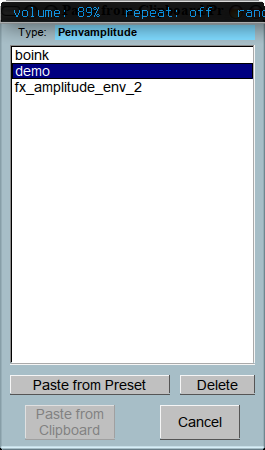
\includegraphics[scale=0.75]{presets/penvamplitude-presets.png}
   \caption{The Penvamplitude Preset}
   \label{fig:presets_penvamplitude}
\end{figure}

   Then click the \textbf{Paste from Preset} button.
   After all this is done, the
   \textbf{Resonance Pad1} sound should 
   be pretty much recovered.
   Pasting the ADDsynth overall preset seems to have the most effect.
   One must play a lot with the presets to fully understand how they work.

   In summary, the presets are essentially keyed to the sub-panels.
   In naming them, you need to use a name that represents the sound that the
   preset contributes, via the settings in its sub-panels.

%-------------------------------------------------------------------------------
% vim: ts=3 sw=3 et ft=tex
%-------------------------------------------------------------------------------
